\documentclass[12pt,a4paper]{article}
\usepackage{amsmath}
\usepackage{mathtext}
\usepackage{icomma}
\usepackage{amsfonts}
\usepackage{amssymb}
\usepackage[utf8]{inputenc}
\usepackage[T1,T2A]{fontenc}
\usepackage[english, russian]{babel}
\usepackage{graphicx}
\usepackage[left=2cm,right=2cm,top=2cm,bottom=2cm]{geometry}
\usepackage{calc}
\usepackage{wrapfig}
\usepackage{setspace}
\usepackage{indentfirst}
\usepackage{subfigure}
\usepackage[table,xcdraw]{xcolor}
\usepackage{float}

\title{Отчет о выполнении лабораторной работы 3.1.3\\
Измерение магнитного поля Земли}

\author{Исламов Сардор, группа Б02-111}
\date{12 ноября 2022 г.}

\begin{document}
\maketitle
\subparagraph*{Аннотация.} В ходе работы определены характеристики шарообразных неодимовых магнитов и, на основе законов взаимодействия магнитных моментов с полем, измерены горизонтальная и вертикальная составляющие индукции магнитного поля Земли и магнитное наклонение.

\subsection*{Теоретическое введение}
\subparagraph*{Точечный магнитный диполь.}
Простейший магнитный диполь может быть образован витком с током или постоянным магнитом. 
По определению, магнитный момент $\overrightarrow{P_m}$ тонкого витка площадью $S$ с током $I$ равен
\[
\overrightarrow{P_m}=\dfrac{I}{c}\vec{S}=\dfrac{I}{c}S\vec{n},
\]
где $\vec{S}=S\vec{n}$ -- вектор площади круга контура. 
Если размеры контура с током или магнитной стрелки малы по сравнению расстоянием до диполя, то соответствующий магнитный диполь называют элементарным или точечным.

Магнитное поле точечного диполя определяется по формуле, аналогичной формуле для поля элементарного электрического диполя:
\[
\vec{B}=\dfrac{3(\overrightarrow{P_m},\vec{r})\vec{r}}{r^5} - \dfrac{\overrightarrow{P_m}}{r^3}
\] 

В магнитном поле с индукцией $B$ на точечный магнитный диполь действует механический момент сил:
\[
\vec{M} = \overrightarrow{P_m}\times \vec{B}.
\]

Под действием вращающего момента $\vec{M}$ виток с током или постоянный магнит поворачивается так, чтобы его магнитный момент выстроился вдоль вектора индукции магнитного поля. 
Это — положение устойчивого равновесия: при отклонении от этого положения возникает механический момент внешних сил, возвращающий диполь к положению равновесия. 
В положении, когда $\overrightarrow{P_m}$ и $\vec{B}$ параллельны, но направлены противоположно друг другу, также имеет место равновесие ($M$ = 0),
но такое равновесие неустойчиво: малейшее отклонение от этого положения приведёт к появлению момента сил, стремящихся отклонить диполь ещё дальше от начального положения.

Магнитный диполь в магнитном поле обладает энергией:
\[
W = -(\overrightarrow{P_m},\vec{B})
\]

В неоднородном поле на точечный магнитный диполь, кроме момента сил, действует ещё и сила:
\[
\vec{F}=(\overrightarrow{P_m},\vec{\triangledown})\vec{B}
\]

Используя формулы для момента силы, силы и энергии, не сложно выяснить, как ведёт себя свободный магнитный диполь в неоднородном магнитном поле: 
он выстраивается вдоль силовых линий магнитного поля и, кроме того, под действием результирующей силы, возникающей из-за неоднородности поля, 
втягивается в область более сильного магнитного поля, т.е. в область, где он обладает меньшей энергией.

Зная магнитные моменты $P_1 = P_2 = P_m$ двух небольших постоянных магнитов, можно рассчитать силу их взаимодействия:
\[
F = P_m \dfrac{\partial B}{\partial r}=-6\dfrac{P_m^2}{r^4}.
\]

\subparagraph*{Неодимовые магнитные шары.}
В настоящей работе используются неодимовые магниты шарообразной формы.
Для нас важно то, что:

1) шары намагничены однородно;

2) вещество, из которого изготовлены магниты, является магнитожёстким материалом.\\

Полный магнитный момент $\overrightarrow{P_m}$ постоянного магнита определяется намагниченностью $\overrightarrow{p_m}$ вещества, из которого он изготовлен. 
По определению, намагниченность – это магнитный момент единицы объёма. 
Для однородно намагниченного шара намагниченность равна:
\[
\overrightarrow{p_m}=\dfrac{\overrightarrow{P_m}}{V}.
\]
 
Намагниченность — важная характеристика вещества постоянных магнитов, определяющая, в частности, величину остаточной магнитной индукции $B_r = 4\pi p_m$. 
Индукция магнитного поля $\overrightarrow{B_p}$ на полюсах однородно намагниченного шара связана с величиной намагниченности и остаточной магнитной индукцией формулами
\[
\overrightarrow{B_p}=\dfrac{8\pi}{3}\overrightarrow{p_m}=\dfrac{2}{3}\overrightarrow{B_r}.
\]

\subsection*{Экспериментальная установка}

\subsubsection*{Определение величины магнитного момента магнитных шариков}

\subparagraph*{Метод А.}
Величину магнитного момента одинаковых шариков можно рассчитать, зная их массу $m$ и определив максимальное расстояние $r_{max}$, на котором они ещё удерживают друг
друга в поле тяжести. При максимальном расстоянии сила тяжести шариков равна силе их магнитного притяжения:

\begin{equation}
    \frac{6P_m^2}{r_{max}^4}=mg \Rightarrow P_m = \sqrt{\frac{mgr_{max}^4}{6}}
\end{equation}

\subparagraph*{Метод Б.}
Если сила сцепления двух одинаковых шаров диаметром $d$ c магнитными моментами $P_m$ равна: $F_0 = \dfrac{6P_m^2}{d^4}$,
то минимальный вес цепочки, при которой она оторвётся от верхнего шарика равен: $F \approx 1.08 F_0$. Тогда\\

\begin{equation}
    P_m = \sqrt{\dfrac{Fd^4}{6.48}}
\end{equation}

\subsubsection*{Определение величины магнитного поля Земли}

\subparagraph*{Горизонтальная составляющая.}

\begin{wrapfigure}{r}{0.22\linewidth}
    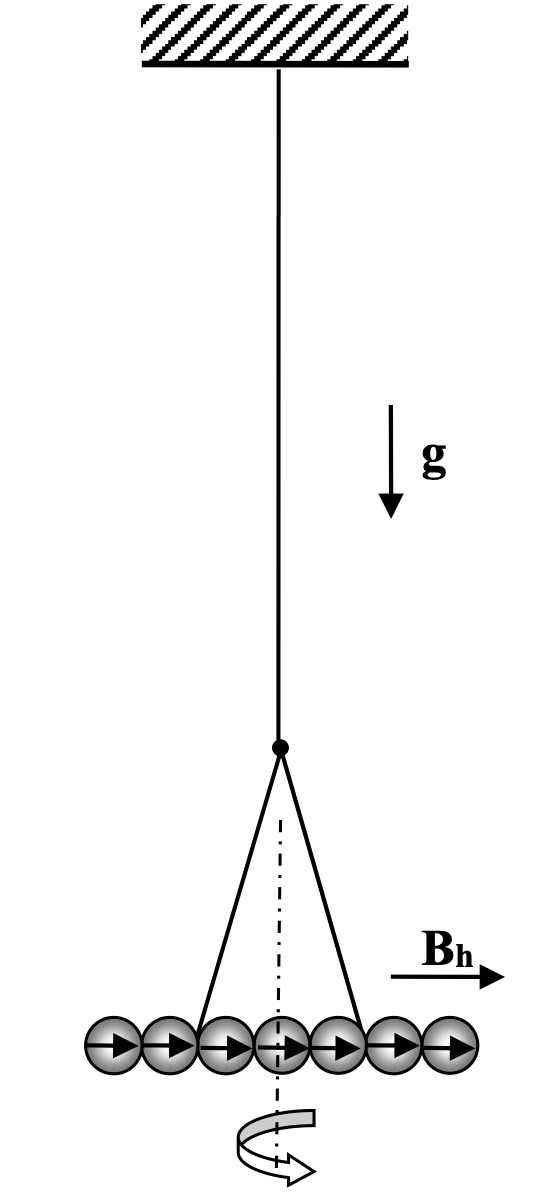
\includegraphics[width=\linewidth]{pics/pic1.png}
\end{wrapfigure}  

Магнитная <<стрелка>> образована из $n$ сцепленных друг с другом противоположными полюсами шариков и с помощью $\Lambda$-образного подвеса подвешена в горизонтальном положении. 
При отклонении «стрелки» на угол $\theta$ от равновесного положения в горизонтальной плоскости возникают крутильные колебания вокруг вертикальной оси, проходящей через середину стрелки. 
При малых амплитудах уравнение колебаний стрелки имеет вид:
\[
I_n \dfrac{d^2 \theta}{dt^2} + P_0 B_h \theta = 0,
\] 
где $P_0$ -- магнитный момент стрелки, $B_h$ -- горизонтальная составляющая магнитного поля Земли, $I_n \approx \dfrac{1}{12}n^3 m d^3$, тогда период колебаний $T = kn$, где $k = \pi \sqrt{\dfrac{md^2}{3P_m B_h}}$. 
Измеряя зависимость $T=T(n)$, находится $B_h$:

\begin{equation}
    B_h = \dfrac{\pi^2 m d^2}{3k^2P_m}
\end{equation}

\begin{wrapfigure}{r}{0.5\linewidth}
    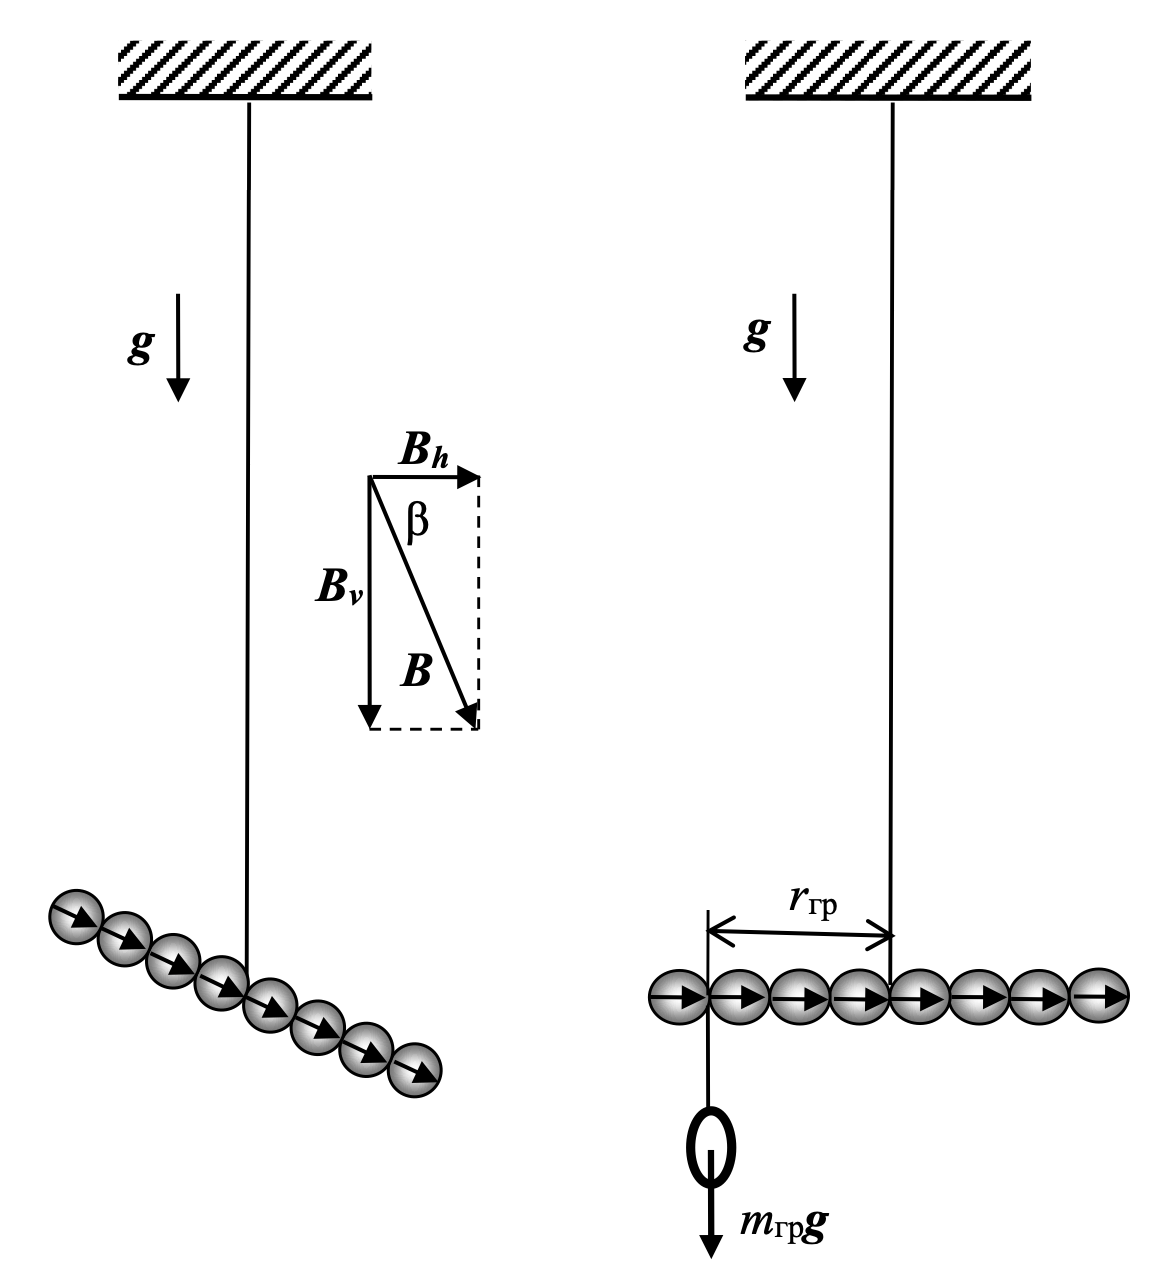
\includegraphics[width=\linewidth]{pics/pic2.png}
\end{wrapfigure} 

\subparagraph*{Вертикальная составляющая.} 
Магнитная «стрелка», составленная из чётного числа шариков и подвешенная на тонкой нити за середину, расположится не горизонтально, а под некоторым, отличным от нуля, углом к горизонту. 
Это связано с тем, что вектор $\vec{B}$ индукции магнитного поля Земли в общем случае не горизонтален, а образует с горизонтом угол $\beta$, зависящим от географической широты $\varphi$ места, где проводится опыт. 
Величина угла $\beta$ называется магнитным наклонением.

С помощью небольшого дополнительного грузика «стрелку» можно «выровнять». 
Момент $M$ силы тяжести уравновешивающего груза пропорционален числу $n$ шариков, образующих магнитную «стрелку» $M(n) = An, A=P_m B_v$, то есть
\begin{equation}
    B_v = \dfrac{A}{P_m}
\end{equation}

\newpage 
\subsection*{Результаты измерений и обработка данных}
\subparagraph*{Метод А.} Измерим массу 12 шариков: $m_{12} = 9.873 \pm 0.001$ г, тогда масса одного шарика $m = (82275 \pm 8) \cdot 10^{-5}$ г.
При этом диаметр, измеренный штангенциркулем равен $d = 5.9 \pm 0.1$ мм.

Подложив между двумя шариками стопку бумаги (непроводящий материал) определим максимальную ширину стопки, при которой шарики все еще удерживают друг друга $h_{max} = 17 \pm 2$ мм.
В таком случае, приравнивая силу взаимодействия двух диполей к силе тяжести шарика, из (1) получаем $P_m = 60 \pm 14$ эрг/Гс. 
Относительная погрешоность составляет около 24\% из-за неточно определяемой ширины стопки.

\subparagraph*{Метод Б.} Теперь определим максимальную массу цепочки, удерживаемой шариками: $m_{max} = 312.192 \pm 0.001$ г. 
В таком случае из (2) получаем $P_m = 76 \pm 2 $ эрг/Гс. 
Как видно, этот способ более точен и предпочтителен для применения в работе.

\subparagraph*{Горизонтальная составляющая магнитного поля Земли}
Измерения и расчеты будем проводить по описанной схеме. 
Соберем крутильный маятник, подвесив «стрелку» из $n$ шариков и измерим период колебаний.
Все измерения в таблице 1. (Первые 3 замера проводились по 10 и по 20 оборотов для проверки стабильности колебаний, далее замеры только по 10 колебаний)

\begin{table}[H]
    \centering
    \begin{tabular}{|l|c|c|c|c|c|c|c|c|c|c|}
    \hline
    n (шарики)   & 3     & 4     & 5     & 6     & 7     & 8     & 9     & 10    & 11    & 12    \\ \hline
    10$T$, с     & 13,01 & 18,05 & 22,65 & 26,24 & 30,86 & 35,26 & 39,58 & 45,09 & 50,23 & 55,12 \\ \hline
    20$T$, с     & 26,09 & 36,12 & 45    &   -   &   -   &   -   &   -   &   -   &   -   &   -   \\ \hline
    $T$, с       & 1,3045& 1,806 & 2,25  & 2,624 & 3,086 & 3,526 & 3,958 & 4,509 & 5,023 & 5,512 \\ \hline
    \end{tabular}
    \caption{Периоды колебаний}
\end{table}

Изобразим зависимость в виде графика (рис. 1):
\begin{figure}[H]
    \centering
    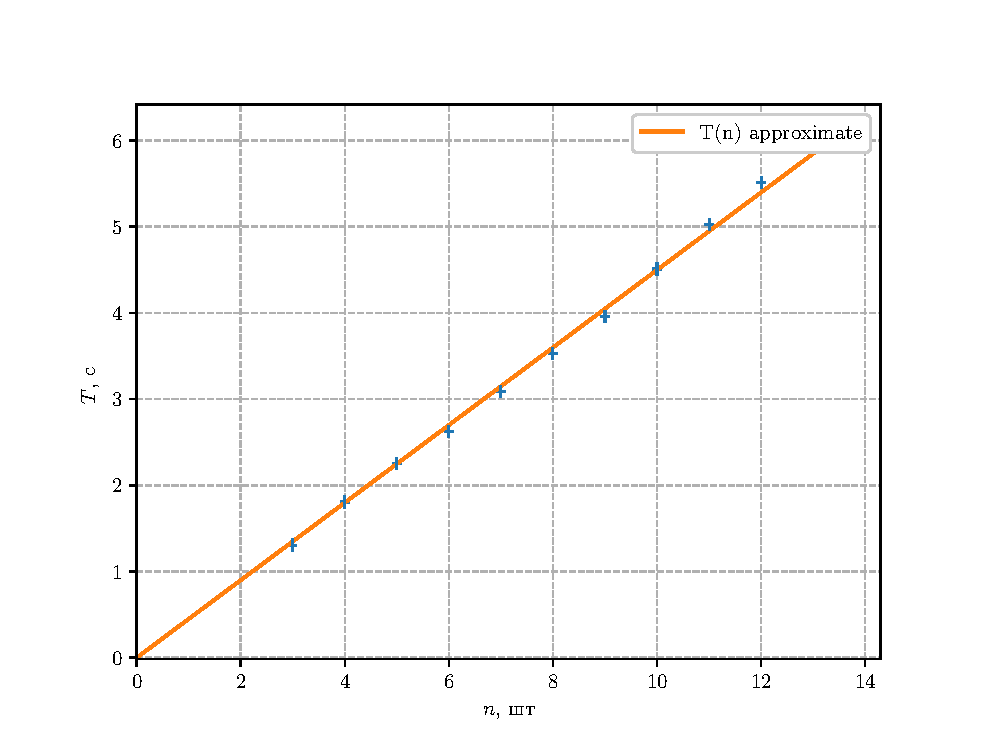
\includegraphics[width=0.75\linewidth]{pics/Tn.eps}
    \caption{Зависимость $T(n)$}
\end{figure}
Угловой коэффициент прямой $k = 0.450 \pm 0.003$.
Теперь по формуле (3) вычислим искомое значение поля: $B_h = (6.1 \pm 0.2) \cdot 10^{-6}$ Тл.
\subparagraph*{Вертикальная составляющая магнитного поля Земли}
Соберем «стрелку» из четного числа шариков $n$, подвесим ее за центр и уравновесим грузиком. 
Данные о грузиках занесем в таблицу 2 (плечо $l$ указано в количестве шариков от центра до точки подвеса груза).
\begin{table}[H]
    \centering
    \begin{tabular}{|l|c|c|c|c|c|}
    \hline
    $n$, шт               & 12     & 10    & 8      & 6      & 4      \\ \hline
    $l$, шт               & 5      & 4     & 3      & 2      & 1      \\ \hline
    $m$, г                & 0,105  & 0,110 & 0,113  & 0,140  & 0,221  \\ \hline
    $M$, дин$\cdot$см     & 303,86 & 254,67& 196,21 &162,06  &127,91  \\ \hline
    \end{tabular}
    \caption{Моменты силы грузов}
\end{table}

Теперь изобразим зависимость на графике (рис. 2):
\begin{figure}[H]
    \centering
    \includegraphics[width=0.75\linewidth]{pics/mn.eps}
    \caption{Зависимость $M(n)$}
\end{figure}
Коэффициент наклона прямой равен $k = 25.7 \pm 0.7$. 
Тогда величина вертикальной составляющей магнитного поля Земли по (4) равна $B_v = (3.39 \pm 0.17) \cdot 10^{-5}\ Тл$, а полная величина поля $B = 0.340 \pm 0.017$ Гс.
Также получаем значение магнитного наклонения $\beta = \arctan{\dfrac {B_v} {B_h}} = 80^о \pm 5^о$.

\subsection*{Подведение итогов}
В ходе работы были получены характеристики шарообразных неодимовых магнитов и, на их основе, вычислено значение магнитного поля $B = 0.340 \pm 0.017$ Гс ($\varepsilon = 5\%$) и магнитного наклонения $\beta = 80^о \pm 5^о\ (\varepsilon = 6\%)$.
Значение поля разнится с табличным значением $B = 0.5$ Гс, в то время как угол совпадает с $\beta = 75\%$, что может свидетельствовать о влиянии железобетонного каркаса здания и излучения окружающих приборов. 
\end{document}